\chapter{Latent Semantic Analysis}
\label{sec:lsa}

\begin{summary}
The chapter gives a theoretical overview of \gls{LSA} in the context of its use in this work.
\end{summary}
 
\section{Information Retrieval process}
\gls{IR} systems aim to satisfy user's information needs, by providing access to large collections of documents.  In a search application, the \gls{IR} process retrieves a set of documents which match a given query. There are three basic processes which an \gls{IR} system has to support: to represent the content of the documents, to represent the user's information need, and to compare the two representations, based on a chosen similarity measure~(Section~\ref{lsa:ir_process}).
%
% IR process
%
\begin{figure}[htbp]
\label{lsa:ir_process}
	\centering
	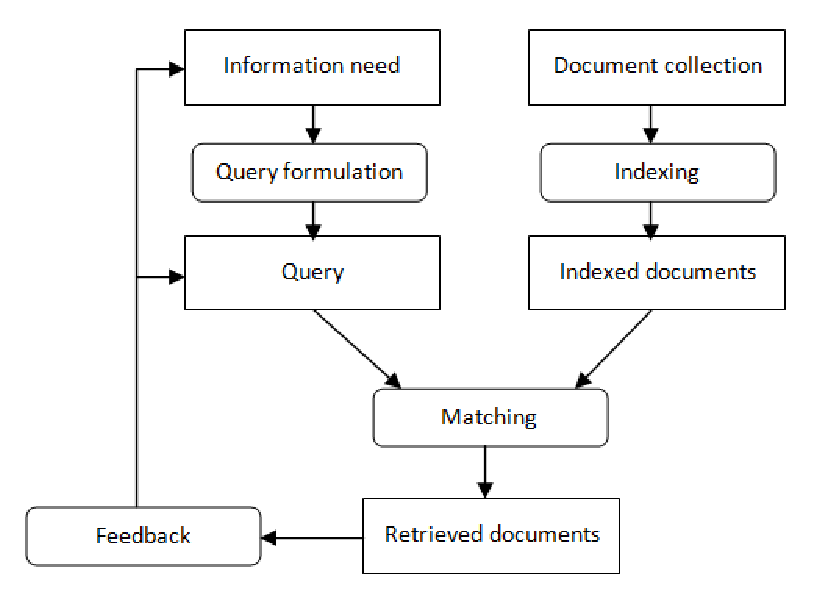
\includegraphics[scale=0.7]{img/IR} 
	\caption[Information Retrieval process]%
           {Information retrieval process, adapted from \cite{IRmodels09}. The information need of the user is formulated as query, which is transformed in the chosen model of the \gls{IR} system. Documents from the collection are likewise represented according to the chosen model. Based on the implemented similarity measure, matching documents are identified. Finally, the retrieval results are presented to the user. If the user is not satisfied with the retrieved result, during feedback the query can be reformulated.}
\end{figure} 
Therefore, the first stage of constructing an \gls{IR} system is to extract information about the documents content, and implement a similarity measure, based on which documents and queries can be compared. Representing the documents is usually called the \textit{indexing process}. The comparison of the query against the document representations based on a chosen measure is called the \textit{matching process}.\\

\section{Document representation}
\label{sec:lsa:doc_repres}
In order to find documents which are similar to a given query, both documents and query have to be comparable, or have the same representation in the \gls{IR} system. Various models have been proposed for internal representation of documents and queries. The \textit{Boolean}, \textit{Vector space} and \textit{Probabilistic} models are popular \gls{IR} models that find wide implementation. The Boolean model represents both documents and queries as a set of terms, and compares them based on boolean functions ($AND$, $OR$, $NOT$, etc.). The probabilistic model uses probabilistic inference for document retrieval~\cite{probabilistic77}. Similarities are computed as probabilities that a document is relevant for a given query. And finally, the \gls{VSM} represents the documents and queries as vectors in a multidimensional space, whose dimensions are the terms used to build an index to represent the documents (subsection \ref{lsa:vsm} provides more details on \gls{VSM}). Boolean model is easy to implement; however, it doesn't offer weighting of terms, leaving all words in the document collection and in the query equally important. When querying, users need to be familiar with boolean operators, which is an additional drawback to this model. The probabilistic model requires prior knowledge, as its implementation usually includes the tuning of independent probabilistic parameters. \gls{VSM} and the probabilistic model both have the advantage that they rank the relevant results according to a chosen weight function, but the former is easier to implement. \\

\subsection{Vector Space Model}
\label{lsa:vsm}
Documents are presented as data structures in memory. In \gls{VSM} a document is a vector, whose elements represent properties like term frequencies, or the frequency of occurrence of words within the document. Before documents can be represented as vectors, they have to be tokenized, or converted from a stream of characters to a stream of words. Thus parsed words will be used in further processing, e.g. in building an index of the document collection. During tokenization one can also apply filtering, i.e. removing HTML tags or other markup from text, as well as stop-words and punctuation marks removal. Stop words are such words that don't convey information specific to the text corpus, but occur frequently, such as: $ a, an, and, any, some, that, this, to $. \\
%
% vsm
%
\begin{figure}[H]
\label{lsa:vsm}
	\centering
	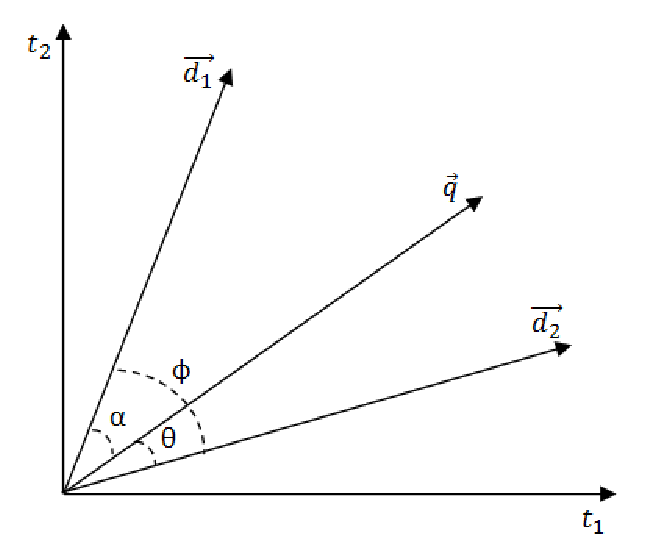
\includegraphics[scale=0.7]{img/vsm} 
	\caption[The Vector Space Model]%
           {The Vector Space Model. Documents $\vec{d_{1}}$ and $\vec{d_{2}}$, and a query vector $\vec{q}$ are represented in a two-dimensional vector space.}
\end{figure}

A distinction has to be made between words or terms, and tokens. A term is the class which is used as a unit during parsing, and a token is each occurrence of this class. For example, in the sentence: 

\begin{quote}
\textit{CoreMedia CMS is shipped with an installation program for interactive graphical installation and configuration of the software.}
\end{quote}

the term $ installation $ is represented by two tokens. \\

There is no universal way in which to parse a text, and the parsing decisions to address depend on the application in which the text collection will be used. \\

After tokenization, documents are represented as vectors, where each term from the document is an element in the vector. Thus, all document vectors and terms form a multi-dimensional vector space, where the terms are the dimensions, and the documents are the corresponding vectors. A representation of the vector space is given in fig.~\ref{lsa:vsm}, where two document vectors $\vec{d_{1}}$ and $\vec{d_{2}}$, and a query vector $\vec{q}$ are represented in a two-dimensional space. \\

\subsection{Weight functions}
\label{lsa:weight_functions}
Vectors in \gls{VSM} have as elements the occurrence frequencies of words in documents. However, some documents are shorter than others, therefore one has to apply a normalization function in order to avoid representing words from longer documents as "more important" than words from shorter documents, as they would occur more often. Such normalization function are called weight functions, and they are applied after the vector space has been constructed. \\

Weight functions are generally separated into two categories - local and global. They are often implemented as a pair together, because local functions measure the importance of a given word in a single document, while global functions give the importance of a word in the whole document collection. The most commonly used functions pair is \textit{term frequency} and \textit{inverse document frequency}. \\

\subsubsection{Term frequency - inverse document frequency}
\label{lsa:tf-idf-section}
The simplest local weight is the term frequency $tf_{t,d}$. It assigns a weight to each term, equal to the number of occurrences of the term $t$ in a given document $d$. However, not all words carry the same meaning in text (therefore we remove the \textit{stop words} during preprocessing, for example~(fig.~\ref{fig:text_analysis}). Words that are common to all documents in the collection don't reveal much information, as compared to words which occur only in several documents. The latter are more likely to contain more information about the meaning of these documents.  This is reflected by the weight function \textit{inverse document frequency}~(eq.~\ref{lsa:idf})
\begin{equation}
\label{lsa:idf}
idf_{t}=1 + log\frac{N}{df_{t}}
\end{equation}

where $N$ is the total number of documents in the collection, and $t$ is a specific term we are weighting. Using $idf_{t}$ is another way to scale down the importance of commonly used words in text. When one combines both $tf$ and $idf$, a composite weight is produced for each term in each document. The \textit{tf-idf} weighting function assings to term $t$ a weight in document $d$ given by 
\begin{equation}
\label{lsa:tf_idf}
(tf-idf)_{t,d}=tf_{t,d} \times idf_{t}
\end{equation}. 

As defined by Manning et al.~\cite{IRbook2008}, the weight assigned to term $t$ in document $d$ is 
\begin{enumerate}
\item highest when $t$ occurs many times within a small number of documents;
\item lower when the term occurs fewer times in a document, or occurs in many documents;
\item lowest when the term occurs in virtually all documents.
\end{enumerate} 

\subsubsection{Log - entropy}
\label{lsa:log-entropy-section}
Another popular pair of weight functions, frequently used in text analysis, is the log-entropy pair. The local function log takes the logarithm of the raw term frequency, thus normalizing the effect when large differences in frequencies occur. In eq.~\ref{lsa:log} $L(t,d)$ denotes the local function giving the weight term $t$ in document $d$. \\
% log
\begin{equation}
L(t,d)=\log(tf(t,d)+1)
\label{lsa:log}
\end{equation}

The global function entropy $H(d,t)$ is the conditional distribution given that term $t$ appeared in document $d$~(eq.~\ref{lsa:entropy}). \\

% entropy
\begin{equation}
G(t) = H(d,t) = 1+\frac{{\Sigma_{j}p(t,d)}}{\log n}
\label{lsa:entropy}
\end{equation}

In eq.~\ref{lsa:entropy}, $p(t,d)$ is defined by:
% entropy
\begin{equation}
p(t,d) = \frac{tf_{t,d}}{gf_{t}}
\end{equation}

where $gf_{t}$ is the total number of times that term $t$ occurred in the whole document collection (in all documents). The entropy measure takes into account the distribution of terms over documents. \\

\subsection{Similarity measures}
\label{lsa:similarity_measures}
Once the vector space has been built, one can find the documents which are most similar to a given query. During \textit{query formulation}(fig.~\ref{lsa:ir_process}), the queries are tokenized and represented as vectors, as already described in section~\ref{lsa:vsm}. Therefore, the similarities between documents and queries can be measured based on the angles between their respective vectors~(in fig.~\ref{lsa:vsm}, these are $ \alpha $ and $ \theta $). Using the angles between vector representations, one can define a similarity measure which is necessary for the matching process in \gls{IR} systems~(fig.~\ref{lsa:ir_process}, as we pointed out. The standard way of computing the similarity between two documents $d_{1}$ and $d_{2}$ is to compute the \textit{cosine similarity} of their vector representations $\overrightarrow{d_1}$ and $\overrightarrow{d_2}$ ~(eq.~\ref{lsa:cosine_measure}).

%
% cosine similarity
%
\begin{equation}
\label{lsa:cosine_measure}
sim(d1,d2)=\frac{\overrightarrow{V}(d_1).\overrightarrow{V}(d_2)}{\left\vert \overrightarrow{V}(d_1) \right\vert.\left\vert \overrightarrow{V}(d_2)\right\vert},
\end{equation}

where the numerator represents the \textit{dot product}\footnote{The dot product $\overrightarrow{x}.\overrightarrow{y}$ of two vectors is defined as $\displaystyle\sum\limits_{i=1}^{M} x_{i}y_{i} $.} of the vectors, while the denominator is the product of their \textit{Euclidean lengths}\footnote{Let $\overrightarrow{d}$ is the document vector for $d$, with $M$ components $\overrightarrow{d_{1}}...\overrightarrow{d_{M}}$. The Euclidean length of $d$ is defined to be $ \sqrt{\sum\limits_{i=1}^{M} \overrightarrow{d_{i}^2}} $}. The measure from eq.~\ref{lsa:cosine_measure} is the cosine of the angle between the two vectors $\overrightarrow{d_1}$ and $\overrightarrow{d_2}$. \\

Viewing a collection of $N$ documents as a collection of vectors leads to a natural view of a collection as a \textit{term-document matrix}: this is an $m \times n$ matrix whose rows represent the $m$ terms (dimensions) of the $n$ columns, each of which corresponds to a document. And this model of representation of a document collection is used in \textit{Latent Semantic Analysis}, a technique which we will discuss next.\\

\section{Latent Semantic Analysis}
Successful though the classic Vector Space Model is, it does not address many of the
problems of modern Information Retrieval. First, the model is based on literal
matching between terms from a document and those of a query. Due to the phenomenon
of synonymy however, there are usually many ways in which the same idea can be expressed
� the terms found in the user's query may not match those of a relevant document.
In this way, some of the documents will not appear in the search results even though they
should. Second, the Vector Space Model model makes an assumption that the keywords
used to index the document collection are mutually independent. Nevertheless, in real
applications it may not always be the case. For this reason significant volumes of redundant
information are present in the classic term-document matrix. And last, the classic
\gls{VSM} uses single words to describe documents while it is the concepts that the majority
of users look for. (??) \\

\gls{LSA} was first introduced~(\cite{Dumais88usingLSA},~\cite{Deerw90_LSA}) as a technique for improving information retrieval. Most search engines work by matching words in a user's query with words in documents. Such information retrieval systems that depend on lexical matching have to deal with two problems: synonymy and polysemy. Due to the many meanings which the same word can have, also called polysemy, irrelevant information is retrieved when searching. And as there are different ways to describe the same concept, or synonymy, important information can be missed. \gls{LSA} has been proposed to address these fundamental retrieval problems, having as a key idea dimension reduction technique, which maps documents and terms into a lower dimensional semantic space. \gls{LSA} models the relationships among documents based on their constituent words, and the relationships between words based on their occurrence in documents. By using fewer dimensions than there are unique words, \gls{LSA} induces similarities among words including ones that have never occurred together~\cite{Dumais2006}. There are three basic steps in using \gls{LSA}: text pre-processing, \gls{SVD} with dimensionality reduction, and querying.\\

\gls{LSA} is based on the \gls{VSM}, representing documents as vectors. ?? \\

After tokenization, one has to construct a term-document matrix~(eq.~\ref{lsa:sparse_matrix_A}). Having as rows the terms, and as columns the documents, its elements are the occurrences of each term in a particular document, where $ a_{ij} $ denotes the frequency with which term $ i $ occurs in document $ j $. The size of the matrix is \text{\bf{m x n}}, where {\bf m} is the number of terms, and {\bf n} is the number of documents in the text collection. Since every term doesn't appear in each document, the matrix is usually sparse. \\

%
% initial sparse matrix A
%
\begin{equation}
A=
\begin{bmatrix}
\label{lsa:sparse_matrix_A}
 a_{11}& a_{12}& \cdots& a_{1n} \\
 \vdots& \vdots& \ddots& \vdots \\ 
 a_{m1}& a_{m2}& \cdots& a_{mn}
\end{bmatrix}
\end{equation}\\

Local and global weightings are applied to increase or decrease the importance of terms within documents. We can write
%
% general weighting function
%
\begin{equation}
\label{lsa:global_local_weighting}
a_{ij}=L(i,j) \times G(i),
\end{equation}

where $L(i,j)$ is the local weighting of the term $i$ in document $j$, and $G(i)$ is the global weighting for term $i$. The choice of a weight function has impact on \gls{LSA} performance, therefore in Section~\ref{sec:lsa:factors_infl_lsa} we give an overview of the most common weight functions. \\

\section{Singular Value Decomposition}
\label{sec:lsa:svd}

After the initial preprocessing, the term-document matrix is decomposed into three matrices~(eq.~\ref{lsa:svd}) by applying \gls{SVD}. It is a unique decomposition of a matrix into the product of three matrices - $U$, $V$ and $\Sigma$, where $U$ and $V$ are orthonormal matrices\footnote{An orthonormal matrix is a matrix, whose columns, treated as 
 vectors, are also orthonormal. A matrix is orthonormal, if its transpose is equal to its inverse. For more information on matrices and matrix operations, refer to~\cite{MatrixCompGolub96}}, and $ \Sigma $ is a diagonal matrix\footnote{A diagonal matrix is a square matrix, in which the entries outside the main diagonal are all $0$.} having singular values\footnote{For a square matrix $A$, the square roots of the eigenvalues of $A^{T}A$, where $A^{T}$ is the conjugate transpose, are called \textit{singular values}. Given a matrix $A$, a non-zero vector $x$ is defined to be an \textit{eigenvector} of the matrix, if it satisfies the \textit{eigenvalue equation}: $Ax=\lambda x$ for some scalar $ \lambda $. The scalar $ \lambda $ is called an \textit{eigenvalue} of $A$ corresponding to the eigenvector $x$.\cite{MatrixCompGolub96}} on its diagonal.\\
%
% SVD decomposition in three matrices
%
\begin{equation}
\label{lsa:svd}
A=U \Sigma V^{T}
\end{equation}

After the initial matrix $A$ is decomposed, all but the highest $k$ values of $\Sigma$ are set to $0$. The resulting reduced matrix represents the semantic space of the text collection. A classical example presenting the truncated \gls{SVD}~(as given in \cite{Dumais88usingLSA}) can be used for displaying dimensionality reduction, and how it affects all three matrices.\\
%
% diagram of the truncated SVD
%
\begin{center}
\begin{figure}[htbp]
\label{lsa:truncated_svd}
	\centering
	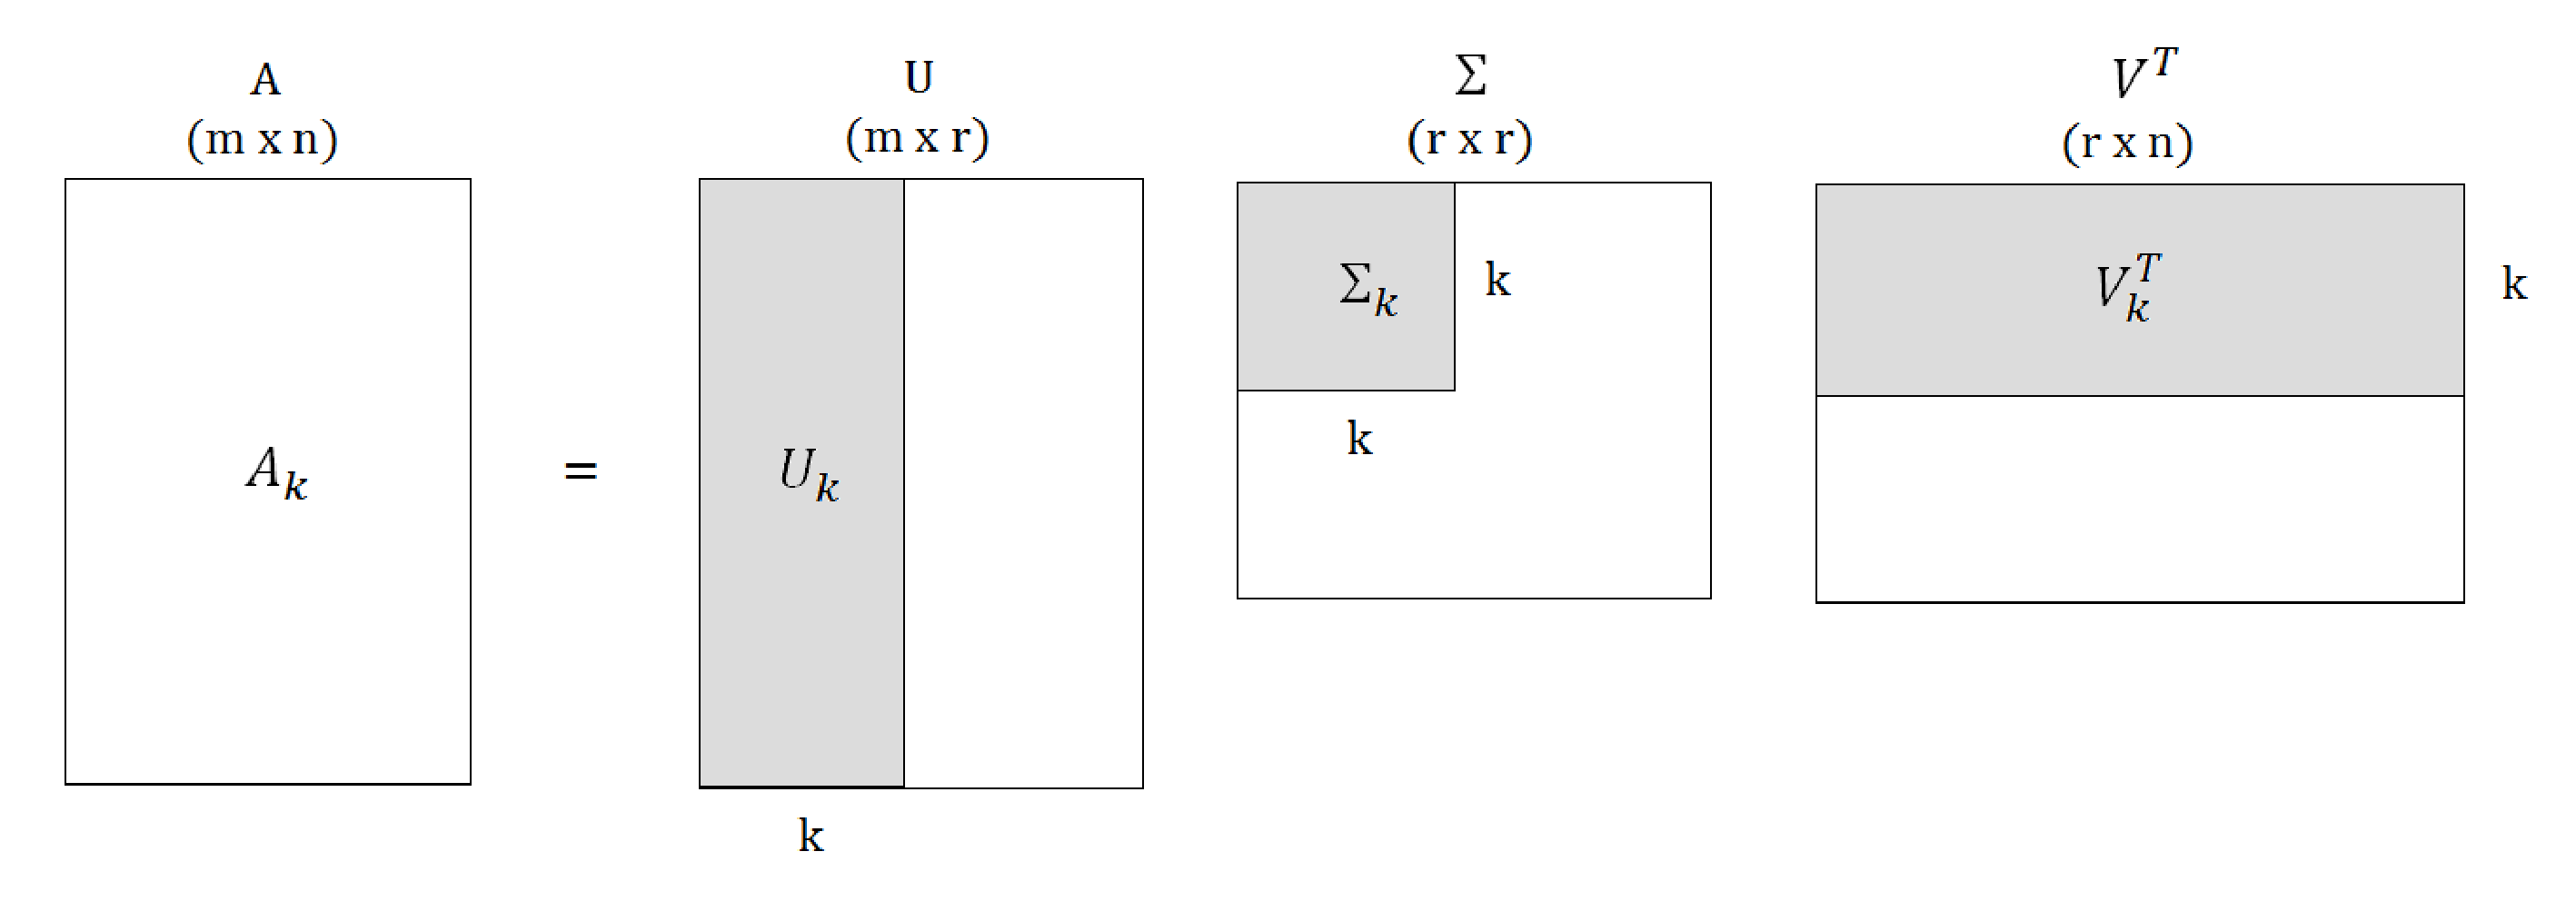
\includegraphics[width=\ScaleIfNeeded]{img/svd} 
 % or [scale=0.5]
	\caption[Diagram of truncated SVD]%
           {Diagram of truncated SVD}
\end{figure}
%
% description of the parameters in SVD diagram
%
\begin{tabular}{l l}
$A_{k}$ - best rank-$k$ approximation of $A$ & $m$ - number of terms\\
$U$ - term vectors & $n$ - number of documents \\
$\Sigma$ - singular values & $k$ - number of factors \\
$V^{T}$ - document vectors & $r$ - rank of $A$ \\
\end{tabular}
\end{center} 

Figure~\ref{lsa:truncated_svd} is a visual representation of \gls{SVD} as defined in equation~(\ref{lsa:svd}). $U$ and $V$ are considered as containing the term and document vectors respectively, and $\Sigma$ is constructed by the singular values of $A$. An important property of \gls{SVD} is that the singular values placed on the diagonal of $\Sigma$ are in decreasing order. Hence, if all but the first $k$ singular values are set to $0$, the semantic meaning in the resulting space is preserved to some approximation $k$, while noise or variability in word usage, is filtered out. Noise in this case are the terms with lowest weights which carry little meaning. By using fewer dimensions $k$, \gls{LSA} induces similarities among terms including ones that have never occurred together. Terms which occur in similar documents, for example, will be near each other in the k-dimensional space even if they never co-occur in the same document. This means that some documents which do not share any words with a users query may be near it in k-space.\\

A factor to be considered when computing \gls{SVD} is the run-time complexity of the algorithm. For decomposition of very large matrices, it is $O(n^2k^3)$, where $n$ is the number of terms in the text corpus, and $k$ is the number of dimensions in semantic space after dimensionality reduction. Note that $k$ is typically a small number between 50 and 350.\\

A more detailed description of \gls{SVD} can be found in \cite{Berry95usinglinear} and \cite{MatrixCompGolub96}.\\

\section{Querying the semantic space}
\label{lsa:querying_sspace}

In this work we are using \gls{LSA} for \gls{IR} purpose. Therefore, the final step of applying the technique is to pose queries on the constructed semantic space. A query $q$ is a set of words which must be represented as a document in the k-dimensional space, in order to be compared to other documents. The user's query can be represented by
%
% Query translation for LSA
%
\begin{equation}
\label{lsa:query}
q = q^{T}U_{k}\Sigma_{k}^{-1}
\end{equation}\\
where $q$ is the set of words in the query, multiplied by the reduced term and singular values matrices. Using the transformation in~eq.~(\ref{lsa:query}), the query is ''mapped'' onto the reduced k-space. After the mapping, the resulting query vector can be compared to the documents in the k-space, and the results ranked by their similarity or nearness to the query. A common similarity measure is the cosine between the query and the document vector. From the resulting document set, the documents closest to the query above certain threshold are returned. \\

\section{Factors which influence LSA performance}
\label{sec:lsa:factors_infl_lsa}
The effective usage of \gls{LSA} is a process of sophisticated tuning. Several factors can influence the performance of the technique. These factors are pre-processing of texts~(removal of stop-words, filtering, stemming), frequency matrix transformations, choice of dimensionality $k$, choice of similarity measure.\\

Dumais et al.~\cite{dumais91improving} and Nakov et al.~\cite{Nakov_weightfunctions} have carried out research on \gls{LSA} performance depending on the choice of factors such as frequency matrix transformations, similarity measures, and choice of dimension reduction parameter $k$. They conclude that performance based on the choice of these factors depends on the particular text corpus, as well as on the purpose of \gls{LSA} application. However, in the case of matrix transform, log-entropy~(section~\ref{lsa:log-entropy-section}) performs better as compared to other matrix transform function combinations, including the popular term frequency - inverse document frequency~($tf-idf$)~(section~\ref{lsa:tf-idf-section}). Therefore, we implement the former in this work. It has been further stated~(\cite{dumais91improving},\cite{NakovBetterResultsLSI}) that with respect to similarity measures used, \gls{LSA} performs optimal when cosine similarity measure~(eq.~\ref{lsa:cosine_measure}) is implemented to calculate the distance between vectors in the semantic space. We have therefore used it to measure the relevance between queries and documents. And finally, the dimensionality reduction parameter $k$ is defined empirically based on the experimentation results presented in Chapter~\ref{sec:implementation}.
